% !TEX root = ../main.tex
% !TEX program = xelatex
\section{问题三的模型建立与求解}

\subsection{日内新信息下的求解思路}

问题三在问题二的基础上增加了新的信息和新的代价。每天0:00先制定购电计划，
6:00、12:00和18:00还能获得新的光伏预报，并允许修改尚未执行的订单，
但修改订单本身需要付费。因此，本问既要判断未来还缺多少电，也要判断是否值得为此修改订单。

当天已经发生的负载同样有用。如果上午用电持续高于零点预测，下午的购电安排就应重新考虑。
不过，一次短暂波动未必会延续到后面，不能把眼前偏差原样加到全天。
光伏预报、实际用电和电池余量需要共同参与下一次决策。

针对这些特点，本文考虑直接使用官方预报、历史融合预报、提升树修正预报，
以及融合预报并增加误差准备四类方案。直接预报最简便；历史融合能够结合当天预报与近期发电水平；
提升树可以表达更复杂的关系；误差准备则着重防范低估缺口后按5倍电价补购的风险。

本文采用\textbf{融合预测与日内校正滚动规划}。
该方案用近期同星期数据判断负载，再用当天已发生的偏差修正后续判断；
光伏由官方预报与历史参考融合得到。在此基础上保留适量准备，
由线性规划权衡普通购电、改单和紧急购电的费用。
这样既能利用新信息，也能说明每次调整的依据。

\subsection{供需预测与动态安全准备}

\subsubsection*{（1）兼顾星期规律与近期变化的负载预测}

负载保留问题二的同星期参照思路，但对较近的日期赋予更高权重。
设 $d$ 为当天，$k$ 为日内第 $k$ 个10分钟时段，零点负载预测为
\begin{equation}
\widehat L^{0}_{d,k}
=\sum_{j=1}^{4}b_jL_{d-7j,k},\qquad
b_j=\frac{0.5^{j-1}}{\sum_{i=1}^{4}0.5^{i-1}}.
\end{equation}
最近四个同星期日的权重依次为 $8/15$、$4/15$、$2/15$ 和 $1/15$。
这一安排保留了星期用电规律，又使近期变化更快进入预测。
只看一周容易受到单日异常影响；四周等权则可能让较早的用电水平影响过大。
四种历史参照的费用比较见后文。

\subsubsection*{（2）用当天已发生的负载修正后续判断}

用 $\tau\in\{0,36,72,108\}$ 表示决策时已经结束的时段数，
分别对应0:00、6:00、12:00和18:00。
在日内决策时，先计算当天已发生时段的平均负载偏差：
\begin{equation}
B_{d,\tau}=\frac{1}{\tau}\sum_{k=1}^{\tau}
\left(L_{d,k}-\widehat L^{0}_{d,k}\right),\qquad \tau>0.
\end{equation}
正偏差表示当天至今的用电高于预期，负偏差则表示低于预期。
随后，将尚未发生的时段按日内时刻划为3小时组，考察过去28个完整日中，
同一决策时刻的已发生偏差与各组后续偏差之间的关系。

设 $Y_{i,\tau,g}$ 为历史日期 $i$ 在未来第 $g$ 组的平均负载预测误差，
$\mathcal H_{d,\tau,g}$ 为可用历史日期集合，则修正系数为
\begin{equation}
\theta_{d,\tau,g}=\operatorname{clip}_{[0,1]}
\left(\frac{\sum_{i\in\mathcal H_{d,\tau,g}}B_{i,\tau}Y_{i,\tau,g}}
{\sum_{i\in\mathcal H_{d,\tau,g}}B_{i,\tau}^{2}}\right).
\end{equation}
该式是无截距最小二乘估计。当天没有偏差时不作额外修正；
历史上偏差延续得越明显，修正比例就越大。
将系数限制在0到1之间，可以避免反向修正或放大短时波动。
有效历史不足7天，或分母接近零时，取 $\theta_{d,\tau,g}=0$。

当天后续负载据此更新为
\begin{equation}
\widehat L_{d,k}^{\tau}
=\max\left\{0,\widehat L^{0}_{d,k}
+\theta_{d,\tau,g(k)}B_{d,\tau}\right\},\qquad k>\tau.
\end{equation}
系数只由此前完整日期估计，当前偏差只使用已经结束的时段。
次日的辅助负载曲线仍由零点已知的同星期历史构造，不直接延续当天偏差。

\subsubsection*{（3）融合官方光伏预报与近期历史}

光伏与负载分别预测。附件3的官方预报按整点给出，本文先在整点融合官方预报与历史参考，
再转换为10分钟序列，以适应购电安排的时间尺度。

以 $\ell$ 表示预报所对应的整点，当前官方光伏预报为 $F_{d,\tau,\ell}$，
近期同钟点的历史参考为 $H_{d,\tau,\ell}$，则整点融合预测为
\begin{equation}
\widetilde P^{PV}_{d,\tau,\ell}
=\lambda_{d,\tau,h}F_{d,\tau,\ell}
+(1-\lambda_{d,\tau,h})H_{d,\tau,\ell}.
\end{equation}
历史参考取该钟点最近7次已结束时段的光伏均值。
这里的 $h$ 按预报提前1--6、7--12、13--18和19--24小时分组。
利用过去28天已经兑现的同组预报，求使平方误差最小的融合权重：
\begin{equation}
\lambda_{d,\tau,h}
=\operatorname{clip}_{[0,1]}
\left(\frac{\sum(F-H)(P^{PV}-H)}{\sum(F-H)^2}\right).
\end{equation}
官方预报近期较准时，其权重增加；历史参考较可靠时，历史信息的比例提高。
因此，融合权重随发布时间和预测提前量变化，而不是全年固定不变。
同组样本不足24条时，合并相同发布钟点的其他提前量样本；仍不足24条，
或分母接近零时，取 $\lambda=1$，直接使用官方预报。

对融合后的相邻整点值作线性插值，得到10分钟光伏预测 $\widehat P^{PV}_{d,\tau,k}$。
决策时刚结束时段的光伏观测作为起点，尚未发生的真实光伏不参与计算。
当前预报只覆盖未来24小时，超过其覆盖范围至次日24:00的辅助时段，采用历史同钟点参考。

\subsubsection*{（4）根据近期净需求误差设置安全准备}

平均预测较准，仍可能在关键时段低估缺口。
少准备的电量可能需要按5倍电价补购，准备过多又可能付费后用不完。
为平衡两者，本文考察历史上实际净需求超过预测的程度：
\begin{equation}
\varepsilon_{i,k}
=\left[(L_{i,k}-P^{PV}_{i,k})
-(\widehat L_{i,k}-\widehat P^{PV}_{i,k})\right]\Delta t.
\end{equation}
历史误差按原发布时间的预测计算，反映当时能够形成的供需判断。

每次决策使用此前28天发布且已兑现的误差，按相同发布时间、目标日内3小时组，
以及预测距发布时间是否达到24小时分别归集。
历史误差采用 $\omega_j\propto0.7^{a_j}$ 的权重，$a_j$ 表示相隔天数。
每早一天权重乘以0.7，约两天降至一半，因而准备量主要跟随近期供需变化。
28天窗口保留四周信息，3小时分组则将每个6小时更新区间分成前后两段。
组内样本不足时合并相同发布时间和覆盖范围的误差，仍不足24条时不附加准备。

取加权误差的0.60分位，并将负值截为零，得到准备量
\begin{equation}
M_{d,\tau,k}=\max\left\{0,Q_{0.60}^{(\omega)}(\varepsilon)\right\}.
\end{equation}
0.60表示误差排序中的位置，不是多买60\%的电，也不是供电保证概率。
它与负载的周权重0.5、误差的日衰减0.7各有不同作用。
分位选得过低容易漏掉缺口，过高则增加无效订电；本问在完整评价期内比较后取0.60。

\subsection{日内滚动购电与储能调度模型}

\subsubsection*{（1）预测供需与决策变量}

为简化表达，以下用 $t$ 连续编号当前时刻至次日24:00的时段，省略日期和发布时间下标。
考虑安全准备后的预计净需求为
\begin{equation}
\rho_t=(\widehat L_t-\widehat P^{PV}_t)\Delta t+M_t,\qquad
N_t=\max(\rho_t,0),\quad A_t=\max(-\rho_t,0).
\end{equation}
$N_t$ 为预计需要外网或电池补充的电量，$A_t$ 为预计可用于储能的光伏富余。
准备量只改变规划中的供需判断；实际运行仍按真实负载与光伏计算。

沿用前文普通订单 $q_t$、外网充电 $x_t$、光伏充电 $y_t$、
电池对外放电 $z_t$ 和内部储电量 $S_t$。
另设 $e_t$ 为预计紧急购电量，$u_t$ 为已订购但预计无法接收的电量。
除 $S_t$ 为电池内部电量外，其余电量均在电池外侧计量。

\subsubsection*{（2）供需平衡与储能约束}

光伏优先直接满足负载后，其余供需满足
\begin{equation}
q_t-x_t+z_t+e_t-u_t=N_t.
\end{equation}
普通订单既能供负载，也能给电池充电。若订单有剩余且电池无法接收，
剩余部分计入 $u_t$，仍按订单付费。

充、放电效率均为90\%，储电量按下式变化：
\begin{equation}
S_t=S_{t-1}+0.9(x_t+y_t)-\frac{z_t}{0.9}.
\end{equation}
容量、功率及电量去向约束为
\begin{equation}
\begin{aligned}
1200&\leq S_t\leq10800,\\
x_t+y_t&\leq P_{\max}\Delta t,\qquad z_t\leq P_{\max}\Delta t,\\
0\leq y_t&\leq A_t,\qquad z_t+e_t\leq N_t,\\
q_t,x_t,y_t,z_t,e_t,u_t&\geq0.
\end{aligned}
\end{equation}
其中 $P_{\max}\Delta t=5000/6\ \mathrm{kWh}$，计算时保留精确值。
这些条件分别限制电池能存多少、每段能充放多少，以及光伏和放电可用于何处。
每次求解的初始库存取当前实际储电量；日末库存连续传递到次日，
不再套用问题一的每日首尾相等条件。

\subsubsection*{（3）订单调整费用}

设零点原始订单为 $q_t^0$，执行前最后确定的订单为 $q_t^F$。
按本文统一采用的结算口径，调减部分退回原计划电费，再收取原电价50\%的违约费；
调增部分支付电费及50\%的附加费。普通订单与调整费用合计为
\begin{equation}
C_{\mathrm{ord}}=\sum_t\left[p_tq_t^F+\frac12p_t|q_t^F-q_t^0|\right].
\end{equation}
例如，100~kWh订单在1元/kWh时减至80~kWh，结算为 $80+10=90$ 元。
同一时段多次调整，只比较最后订单与零点订单的净变化，重叠部分不重复收费。
该式也包含未能接收的普通订单费用，不能只按实际使用量结算。

\subsubsection*{（4）目标函数}

每次规划都延伸至次日24:00，使模型考虑留电对下一天的作用。
记 $\mathcal T_{\tau}$ 为全部规划时段，$\mathcal A_{\tau}$ 为其中当天尚未执行、
且已经在零点订过电的时段。零点决策时 $\mathcal A_0$ 为空。
目标函数为
\begin{equation}
\min J=\sum_{t\in\mathcal T_{\tau}}(p_tq_t+5p_te_t)
+\frac12\sum_{t\in\mathcal A_{\tau}}p_t\delta_t-\nu S_T,
\end{equation}
其中，对 $t\in\mathcal A_{\tau}$ 有
\begin{equation}
\delta_t\geq q_t-q_t^0,\qquad
\delta_t\geq q_t^0-q_t,\qquad\delta_t\geq0.
\end{equation}
只有当日已有订单的修改产生调整费。次日订单只是辅助规划，不在本次签订，也不收调整费。

末端库存系数取 $\nu=0.9p_{0:00}=0.38484$ 元/kWh，
以一度内部存电经放电后可替代的低价外网电作为参考。
$-\nu S_T$ 用于抑制规划末端放空电池的倾向，不是实际售电收入，不计入最终购电账单。
目标函数与约束均为线性关系，故采用线性规划求解。

\subsection{日内滚动求解过程}

每天0:00，模型读取已有历史、当前储电量和官方预报，形成负载、光伏预测与安全准备，
求解得到当天原始购电计划。次日的辅助曲线只帮助判断当前应留多少电。

在6:00、12:00和18:00，先根据已发生的负载计算偏差，修正当天后续负载；
再融合新光伏预报，更新准备量，并从当前真实库存重新求解。
已经执行的订单保持不变，未执行部分是否调整由费用权衡决定。

实际运行以真实供需为准。光伏优先供负载，普通电不足时由电池补充；
达到库存或放电功率限制后，剩余缺口才采用紧急购电。
多余电量在容量和充电功率允许时储存，无法利用的部分不产生售电收益。
日末按最终订单完成结算，实际剩余电量传递至下一天。

费用评价期为2025年2月1日至12月31日，共334天。
各日连续运行，完整方案每天求解4次，共完成1336次滚动线性规划。

\subsection{候选方案比较与最终模型选择}

为区分光伏预测方法的作用，先固定四周同星期等权负载、不作日内负载校正，
且不附加误差准备，只比较三种光伏处理方式。
各方案采用相同的设备、起始库存和结算规则，结果如表~\ref{tab:q3_candidate}所示。

\begin{table}[H]
\centering
\caption{固定负载与准备条件下的光伏预测方案比较}
\label{tab:q3_candidate}
\begin{tabular}{lrrr}
\toprule
光伏处理方式 & 普通结算/万元 & 紧急购电/万元 & 总费用/万元\\
\midrule
直接采用官方预报 &1289.96&127.56&1417.51\\
历史误差融合预报 &1276.36&132.51&1408.87\\
提升树修正预报 &1279.46&136.80&1416.26\\
\bottomrule
\end{tabular}
\end{table}

历史融合的总费用最低，说明官方预报与近期历史能够相互补充。
提升树虽能表达复杂关系，却未在该比较中带来更低费用。
同时，融合方案的紧急购电费仍较高，说明仅改善平均预测并不足以防范缺口，
还需把误差准备纳入购电决策。

负载方面，在同样使用日内校正、融合光伏和0.60分位准备的条件下，
比较一周参照、两周等权、四周等权及四周近期加权，结果见表~\ref{tab:q3_load_compare}。
各方法均由自身的历史预测误差计算准备量，使准备程度与预测方法相匹配。

\begin{table}[H]
\centering
\caption{同星期负载参照方式的费用比较}
\label{tab:q3_load_compare}
\begin{tabular}{lrr}
\toprule
负载参照方式 & 总费用/万元 & 紧急购电/万元\\
\midrule
最近一周 &1306.22&18.82\\
最近两周等权 &1303.74&17.85\\
最近四周等权 &1304.61&15.68\\
\textbf{最近四周近期加权} &\textbf{1301.42}&\textbf{16.13}\\
\bottomrule
\end{tabular}
\end{table}

四周近期加权取得最低总费用，较四周等权节省约3.20万元。
它保留较长历史以平滑单日异常，又能较快跟随近期用电变化。
不过，其紧急购电费略高于四周等权，说明最低总费并不等于每项费用都最低。
本文选择该方案，是在普通订电与紧急补购之间取得更经济的平衡。
两组比较分别支持历史融合与近期加权负载，二者共同用于本问的滚动规划。

\subsection{全年结果与指定日期分析}

\subsubsection*{（1）全年费用结果}

最终方案在334天内的普通订单费为1257.23万元，调整费为28.06万元，
二者合计普通结算费1285.29万元；紧急购电费为16.13万元。
总购电费用为
\begin{equation}
\boxed{C=13014172.33\ \text{元}}.
\end{equation}
评价期内紧急购电量为28627.32~kWh，共185天出现紧急购电。
图~\ref{fig:q3_monthly}给出各月费用构成，4月最低，12月最高。大部分支出来自普通结算，
紧急补购虽电量较少，却需要承担较高单价。

\begin{figure}[H]
\centering
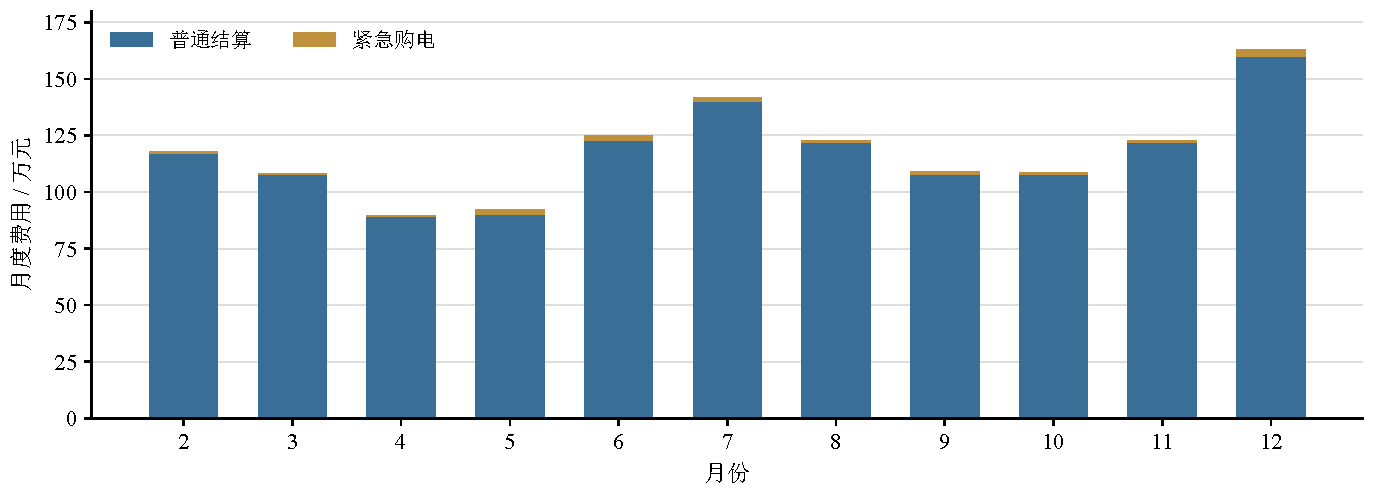
\includegraphics[width=0.95\textwidth]{fig/q3_final_monthly.pdf}
\caption{各月普通结算与紧急购电费用}
\label{fig:q3_monthly}
\end{figure}

安全准备也有代价。全年仍有32.66万kWh普通订单未能接收，
这部分电虽未使用，却已经付费。因此，不能只以紧急购电少作为方案优劣的标准，
还要看为此多付出的普通订电费用。

\subsubsection*{（2）指定日期零点原计划}

题目指定日期在0:00制定的部分购电计划见表~\ref{tab:q3_original_order}。
表中每项均为对应10分钟区间的电量，原计划在当天后续决策中保留，作为调整计费的基准。
% Generated from saved final Q3 trajectories. Do not hand-edit numbers.
\begin{table}[H]
\centering
\caption{指定日期零点原计划的部分时段购电量（kWh）}
\label{tab:q3_original_order}
\small
\setlength{\tabcolsep}{5pt}
\begin{tabular}{lrrrr}
\toprule
时间段 & 3月20日 & 6月21日 & 9月23日 & 12月21日 \\
\midrule
10:00--10:10 & 0.00 & 0.00 & 0.00 & 0.00 \\
12:00--12:10 & 568.44 & 0.00 & 424.94 & 957.12 \\
14:00--14:10 & 0.00 & 0.00 & 0.00 & 0.00 \\
16:00--16:10 & 480.78 & 115.62 & 443.64 & 798.21 \\
18:00--18:10 & 722.54 & 426.86 & 810.48 & 727.22 \\
20:00--20:10 & 0.00 & 0.00 & 0.00 & 0.00 \\
\bottomrule
\end{tabular}
\end{table}


\subsubsection*{（3）日内调整后的购电结果}

经过三次日内决策后，最终普通订单及全天费用见表~\ref{tab:q3_final_order}。
这里的最终订单是该区间执行前最后确定的总量，并非相对零点的增减量。
零点计划与最终订单的差异反映了新供需判断和当前库存对后续安排的影响。
% Generated from saved final Q3 trajectories. Do not hand-edit numbers.
\begin{table}[H]
\centering
\caption{指定日期调整后订单及全天费用（时段订单单位为kWh）}
\label{tab:q3_final_order}
\small
\setlength{\tabcolsep}{5pt}
\begin{tabular}{lrrrr}
\toprule
项目 & 3月20日 & 6月21日 & 9月23日 & 12月21日 \\
\midrule
10:00--10:10 & 0.00 & 0.00 & 0.00 & 0.00 \\
12:00--12:10 & 574.44 & 0.00 & 422.94 & 985.17 \\
14:00--14:10 & 0.00 & 0.00 & 0.00 & 0.00 \\
16:00--16:10 & 480.78 & 71.01 & 443.64 & 827.19 \\
18:00--18:10 & 722.54 & 415.06 & 810.48 & 727.30 \\
20:00--20:10 & 0.00 & 0.00 & 0.00 & 0.00 \\
\midrule
全天原计划购电量/kWh & 62950.87 & 40273.79 & 67565.05 & 94803.82 \\
全天最终普通订单/kWh & 62434.82 & 40006.24 & 67338.24 & 95848.96 \\
全天紧急购电量/kWh & 18.54 & 0.00 & 242.51 & 73.49 \\
普通结算费用/元 & 39514.95 & 22010.94 & 42247.91 & 62215.35 \\
紧急购电费用/元 & 117.15 & 0.00 & 1277.76 & 334.35 \\
全天总费用/元 & 39632.09 & 22010.94 & 43525.66 & 62549.70 \\
\bottomrule
\end{tabular}
\end{table}

前三个日期的最终订单低于零点计划，12月21日则增加约1045~kWh，
说明日内调整并非统一加量或减量，而是随供需判断变化。
表中各项分别四舍五入，费用合计由未舍入值计算。

\subsubsection*{（4）指定日期储能运行}

四个指定日期的实际充放电和日首尾库存见表~\ref{tab:q3_storage}。
充电量在电池输入侧计量，放电量在输出侧计量，首尾库存则为电池内部电量。
某个4小时区间同时有充电和放电，表示内部不同10分钟时段采取了不同动作，
不表示同一时段同时充放电。
% Generated from saved final Q3 trajectories. Do not hand-edit numbers.
\begin{table}[H]
\centering
\caption{指定日期的实际充放电及日首尾储电量（kWh）}
\label{tab:q3_storage}
\small
\setlength{\tabcolsep}{5pt}
\begin{tabular}{llrrrr}
\toprule
时间段 & 项目 & 3月20日 & 6月21日 & 9月23日 & 12月21日 \\
\midrule
00:00--04:00 & 充电 & 1510.42 & 267.18 & 2048.71 & 1958.12 \\
 & 放电 & 238.58 & 302.32 & 61.89 & 239.38 \\
04:00--08:00 & 充电 & 1034.68 & 536.17 & 529.10 & 1617.46 \\
 & 放电 & 5467.56 & 1753.56 & 6328.62 & 793.91 \\
08:00--12:00 & 充电 & 4061.01 & 10134.27 & 4352.49 & 4419.79 \\
 & 放电 & 3259.44 & 0.00 & 2369.61 & 8608.93 \\
12:00--16:00 & 充电 & 6377.03 & 299.24 & 6833.50 & 8730.87 \\
 & 放电 & 254.72 & 0.00 & 417.27 & 2012.03 \\
16:00--20:00 & 充电 & 147.87 & 83.04 & 94.47 & 0.95 \\
 & 放电 & 4675.69 & 5205.83 & 5101.73 & 4983.07 \\
20:00--24:00 & 充电 & 4148.71 & 8559.86 & 8245.77 & 8334.82 \\
 & 放电 & 3749.74 & 3041.10 & 3620.94 & 3624.47 \\
\midrule
0:00 & 内部储电量 & 8871.16 & 2971.14 & 8609.68 & 8695.56 \\
24:00 & 内部储电量 & 4816.54 & 9415.36 & 8614.36 & 8738.25 \\
\bottomrule
\end{tabular}
\end{table}


\subsubsection*{（5）紧急购电与典型日期分析}

指定日期发生紧急购电的时段见表~\ref{tab:q3_emergency}，未列出的时段为零。
6月21日没有紧急购电；其余日期的缺口也并非都由库存触底造成。
% Generated from saved final Q3 trajectories. Do not hand-edit numbers.
\begin{table}[H]
\centering
\caption{指定日期发生紧急购电的时段及电量}
\label{tab:q3_emergency}
\small
\setlength{\tabcolsep}{5pt}
\begin{tabular}{llr}
\toprule
日期 & 时间段 & 紧急购电量/kWh \\
\midrule
3月20日 & 10:00--10:10 & 6.12 \\
 & 20:40--20:50 & 12.42 \\
6月21日 & 无 & 0.00 \\
9月23日 & 09:40--09:50 & 4.35 \\
 & 09:50--10:00 & 13.98 \\
 & 20:30--20:40 & 6.38 \\
 & 20:40--20:50 & 58.51 \\
 & 21:00--21:10 & 65.38 \\
 & 21:10--21:20 & 28.13 \\
 & 21:20--21:30 & 2.38 \\
 & 21:30--21:40 & 34.04 \\
 & 21:40--21:50 & 20.86 \\
 & 21:50--22:00 & 8.51 \\
12月21日 & 08:00--08:10 & 22.46 \\
 & 10:50--11:00 & 51.03 \\
\bottomrule
\end{tabular}
\end{table}


图~\ref{fig:q3_days}展示3月20日和9月23日的供需与储能过程。
3月20日两次补购均发生在电池降至最低库存时。
9月23日20:30，电池虽有余电，当段却已达到最大放电功率，仍需紧急补购；
随后多个时段又因库存触底而补购。

\begin{figure}[H]
\centering
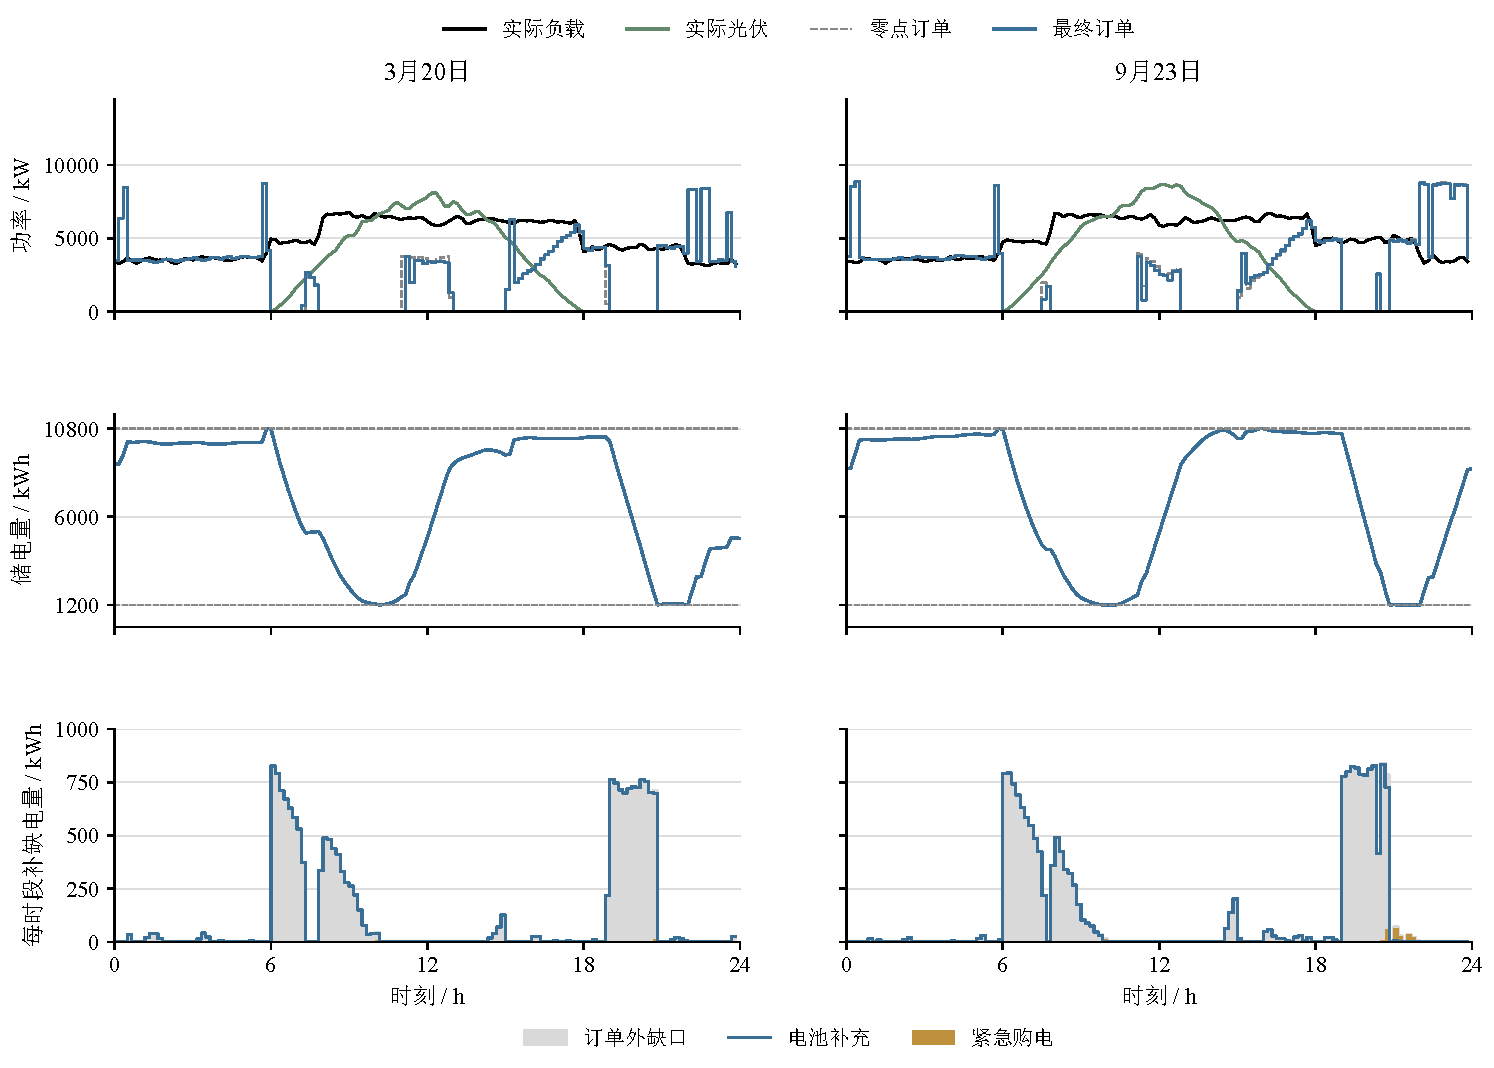
\includegraphics[width=0.98\textwidth]{fig/q3_final_days.pdf}
\caption{两个指定日期的供需、储电状态及缺口补充}
\label{fig:q3_days}
\end{figure}

这说明电池里有电，并不等于任何时段都能及时供够。
判断紧急购电是否必要，必须同时考虑缺口出现的时刻、可用库存和放电功率，
不能只比较全天电量总和。

\subsection{日内新预报的实际费用价值}

题目最后要求判断是否需要引入6:00、12:00和18:00的新光伏预报。
对此，不能把完整方案相对零点固定计划的全部节省都归功于新预报，
因为日内观察实际负载、更新库存和修改订单本身也能改善安排。

本文在同一套负载预测、准备规则和调度结构下设置三组信息条件，
共同从同一实际库存开始连续运行。第一组只在零点订电，全天不改单；
第二组允许根据已发生的供需和库存调整，但不读取后发官方预报；
第三组在第二组基础上加入后发官方预报。
各组的预测误差与准备量均由自身可用信息构造，结果见表~\ref{tab:q3_info}。

\begin{table}[H]
\centering
\caption{同一模型下三种信息条件的费用比较}
\label{tab:q3_info}
\begin{tabular}{lr}
\toprule
信息与决策条件 & 总费用/万元\\
\midrule
零点订电，全天不修改订单 &1359.00\\
日内反馈与改单，不使用后发官方预报 &1308.37\\
日内反馈与改单，使用后发官方预报 &1301.42\\
\bottomrule
\end{tabular}
\end{table}

日内反馈与改单使费用减少50.63万元；在此基础上，
新光伏预报又节省6.95万元，降幅约0.53\%。
后两组期末库存相同，因此这部分节省不是靠多消耗剩余电量换来的。
新增预报的作用虽小于日内反馈与改单的合计作用，仍带来正的费用收益。

\begin{figure}[H]
\centering
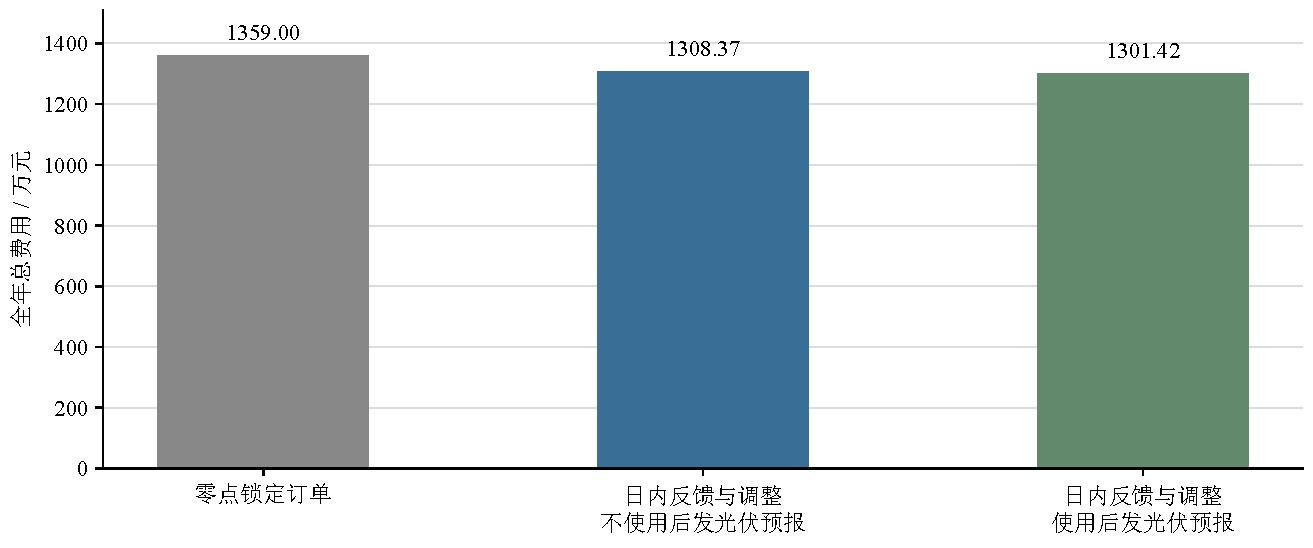
\includegraphics[width=0.90\textwidth]{fig/q3_final_information.pdf}
\caption{日内反馈与后发光伏预报各自带来的费用改善}
\label{fig:q3_info}
\end{figure}

因此，在题目未另计预报获取费用的条件下，\textbf{应引入日内新预报作为决策依据}。
但它不是每次都能省钱：逐日对照中，209天费用降低，125天增加。
收到新预报后是否改单，仍应由预期缺口、调整费用和储能余量共同决定，
不能把“使用预报”理解为“每次必须修改订单”。

\subsection{参数灵敏度与模型可信度}

为考察准备程度是否合适，保持负载与光伏预测、调度方式和结算规则不变，
将误差分位依次取0.40、0.50、0.60、0.70和0.80。
图~\ref{fig:q3_parameter}显示，总费用随准备程度先降后升，0.60在所比较取值中最低。

\begin{figure}[H]
\centering
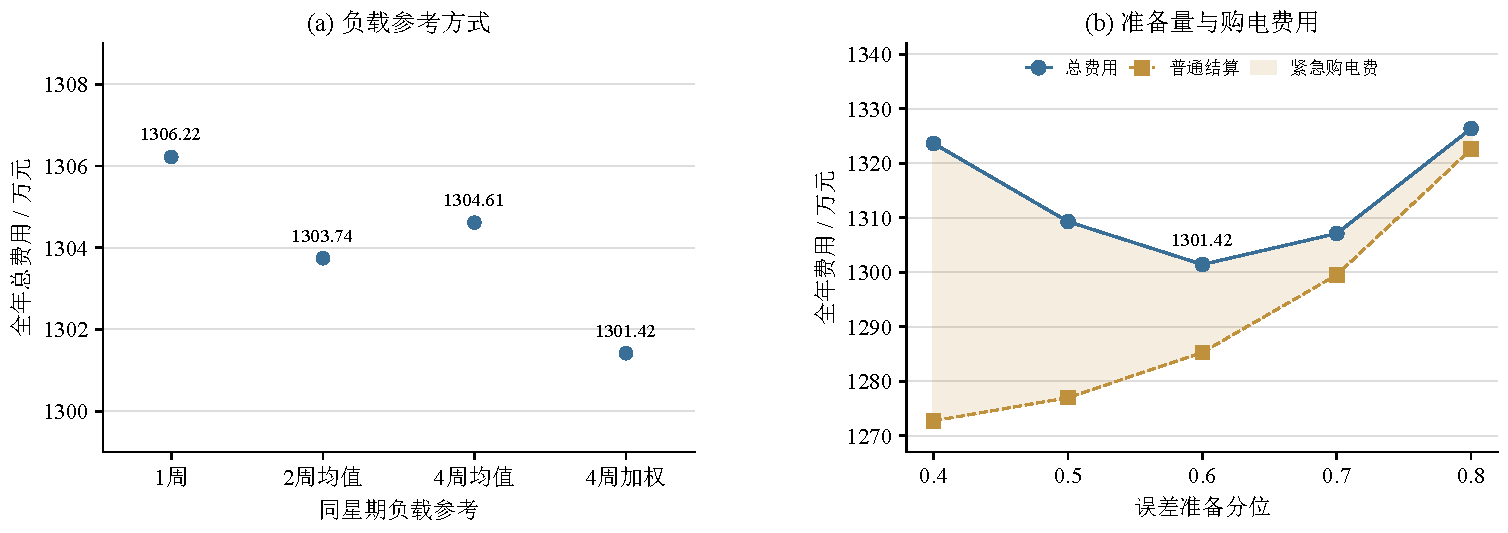
\includegraphics[width=0.96\textwidth]{fig/q3_final_validation.pdf}
\caption{负载参照与误差准备程度的费用比较}
\label{fig:q3_parameter}
\end{figure}

准备不足时，紧急补购抵消了少订普通电的节省；继续增加准备，
虽然能够进一步减少紧急购电，但普通订单和无法接收的电量随之上升。
例如，分位从0.60提高到0.70后，紧急购电费减少约8.54万元，
普通结算费却增加约14.23万元，总费用反而更高。
因此，0.60体现的是本题成本条件下的取舍，并不是准备越多越可靠、越经济。

计算后逐10分钟核对了供需平衡、库存衔接、充放电功率和已执行订单锁定，
并由实际订单与紧急购电量重新计算账单。
各项约束得到满足，费用复算差异小于0.01元。
这能够支持结果在既定信息与结算条件下的可行性，但不能将预测调度的全年费用称为全局最优值。

上述权重与分位在2025年数据内比较，实际决策逐日只读取当时已知信息。
这支持本年度的模型选择，不等于已经证明跨年泛化能力。
用于其他年份或其他微网时，仍需依据新的用电习惯和误差分布重新校准。
